%!TEX root = ../thesis.tex
%*******************************************************************************
%****************************** Third Chapter **********************************
%*******************************************************************************
\chapter{System Architecture}

% **************************** Define Graphics Path ****************************
\ifpdf
	\graphicspath{{Chapter3/Figs/Raster/}{Chapter3/Figs/PDF/}{Chapter3/Figs/}}
\else
	\graphicspath{{Chapter3/Figs/Vector/}{Chapter3/Figs/}}
\fi

\section{Introduction}
% Waar gaat dit hoofdstuk over?

The price calculation system that is being made should integrate in the existing architecture seamlessly. This chapter aims to answer question number three, and its subquestions. First it is determined whether the frontend and backend that are to be developed should be integrated in existing projects, or should be made in separate projects altogether. If the backend is created as a separate project, authentication and authorization are directly affected by these decisions. Separation implies more complex identity management, or less separation of concern. Then, the database should be capable of storing geometry, and accept queries to determine which polygons contain a set of points, and which points are contained within a polygon.

\section{Architectural Patterns}

The current system architecture consists of three public API's and eight private API's that connect to four databases. \mynote{Refer to figure} The core API is the interface to which mobile applications make requests. It is possible to integrate the pricing system as a module in the existing project. This simplifies authentication and authorization, because it already exists is that project. Another option is to implement the system as a microservice, which is infamously known as a service-oriented architecture (SOA). Advantages of a microservice are the fact that a microservice is a self-contained and naturally modular structure, but authentication and authorization must be handled by the microservice itself, unless state is shared amongst services.

\begin{figure}[ht!]
	\centering
	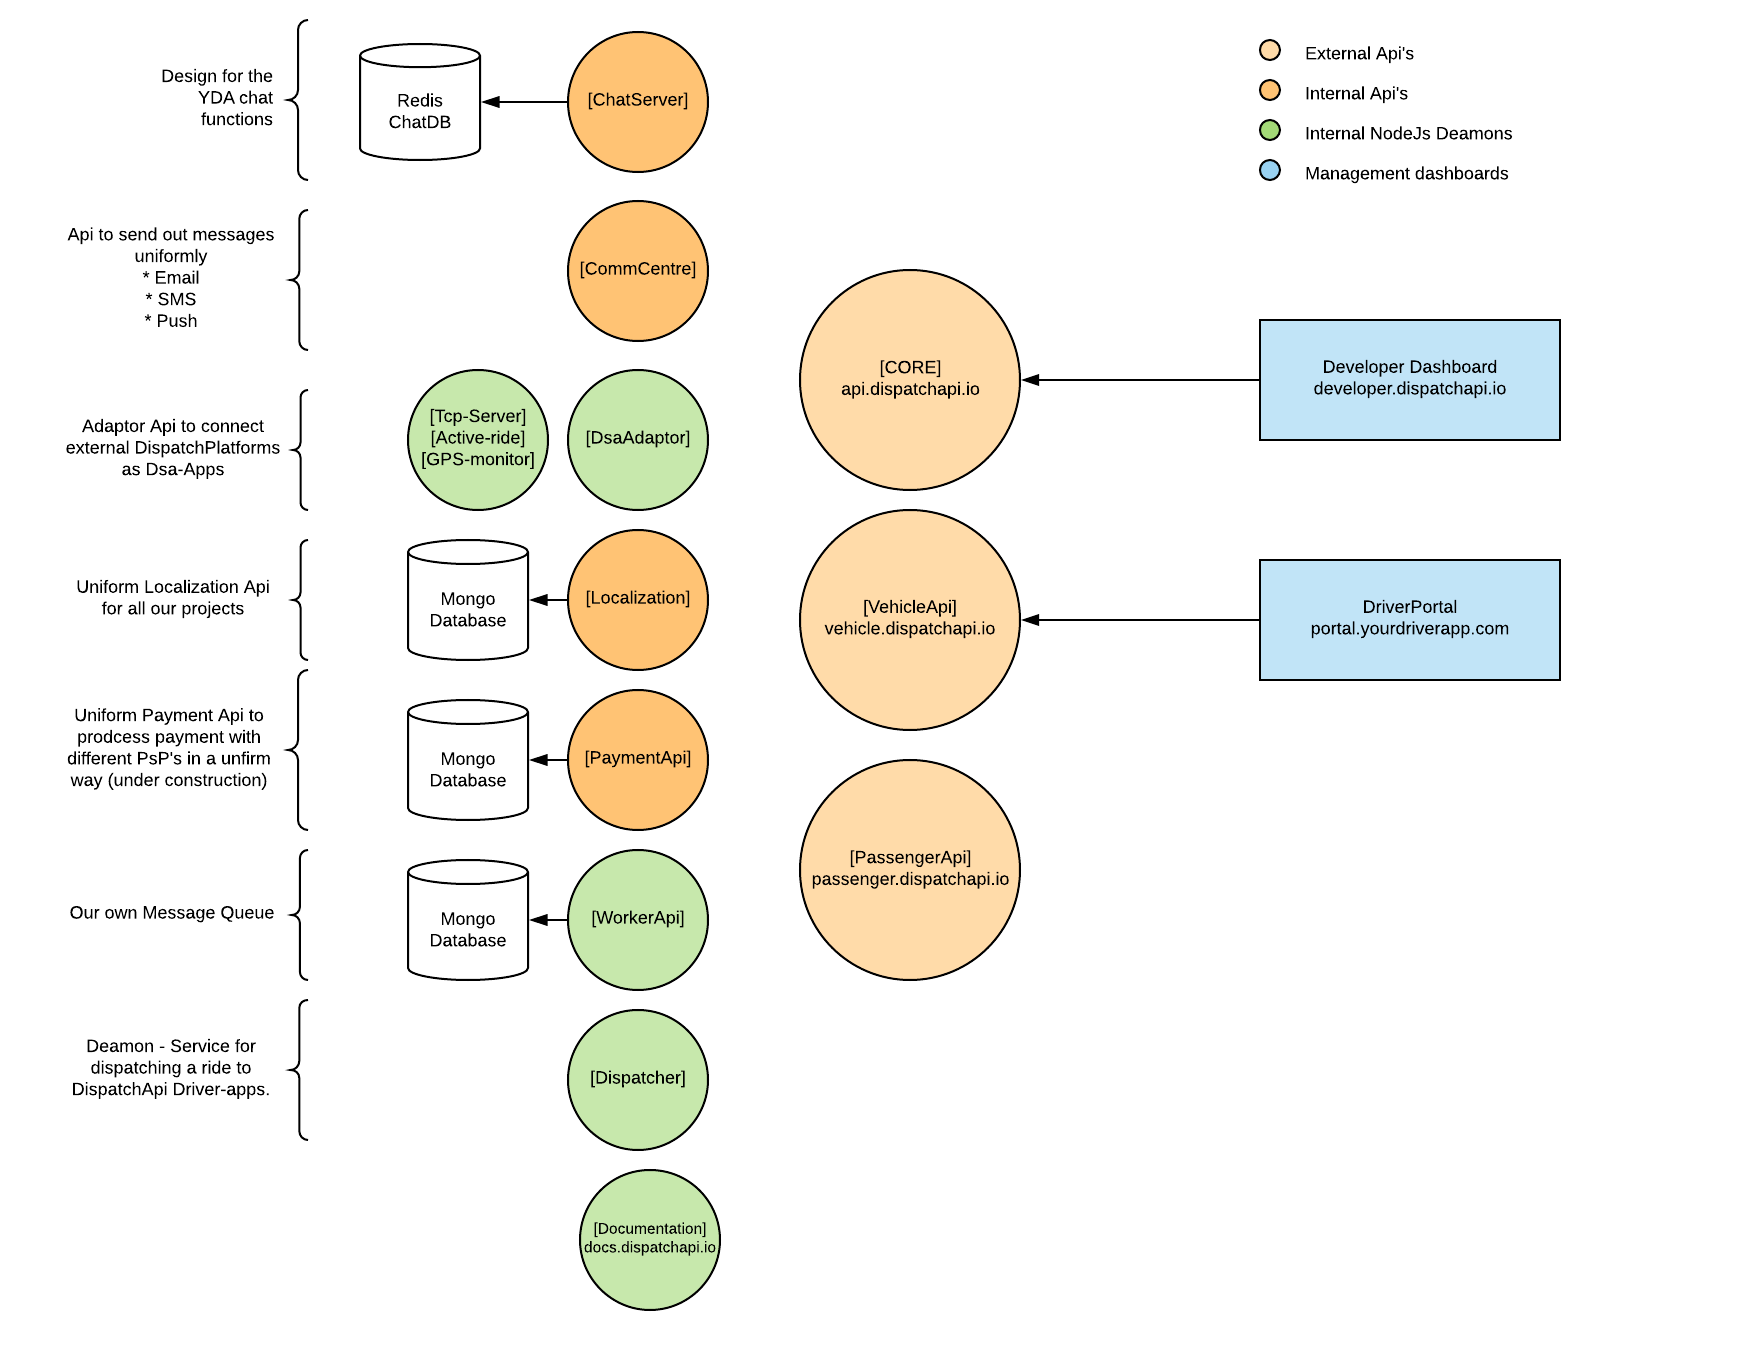
\includegraphics[width=1\textwidth]{Architecture}
	\caption[Architecture]{Current System Architecture}
	\label{fig:Architecture}
\end{figure}
\clearpage


\section{Authentication and Authorization}

Mobile applications should be able to make requests, just like the portals that are to be developed. But portal users make use of the microservice in a different way. Mobile apps merely request prices of products, based on the rules that group admins define through the portal. To make sure that only the portal users have the right to mutate their data, users have to be authenticated and authorized within the microservice. Identity management becomes a problem if data duplication is not desired. If a user makes a direct request to the microservice, the credentials have to be compared to user data in a database. To prevent duplication, the microservice could be connected to the database that is used by the core system. But this makes the microservice less decoupled, and directly contradicts the desire to separate concerns. Four examples demonstrate this problem:

\begin{itemize}
	\item Example 1: The microservice authenticates and authorizes users all by itself, managing sessions and storing user data in its database.
	\item Example 2: The microservice connects to an exising databases to acquire the required information about the user.
	\item Example 3: The core system authenticates the user and provides a token that can be verified by the microservice, containing user identity.
	\item Example 4: A separate service is used for authentication and authorization so that the core system is not involved at all.
\end{itemize}

In the first example, the microservice seems to be independent, because it has knowledge about the users identity without making requests to adjecent systems, or connecting to external databases. But this is not true. If data about the user is mutated in the core system, the microservice needs to be notified or synced. This greatly hinders scaling and makes it harder to keep data consistent. Example two solves the inconsistency part by connecting to the central database that holds user data, but contradicts the strive for encapsulation. Example three entirely removes the database connection to any user data. This is possible when a JSON Web Token (JWT) is used for example. The identity is stored in the token itself as an encrypted payload that can only be revealed by whoever holds the secret with which it was signed. Example four delegates managing user identity to a separate authentication service that, similar to the pricing microservice, has its own single task.


Which architectural pattern is best suited for implementing the pricing system?
\begin{enumerate}
	\item Which architectural patterns fit in with the exising architecture?
	\item How will authentication be handled?
\end{enumerate}
